\documentclass[10pt]{beamer}
\usepackage{SexySlides1,fancyvrb,outlines,pbox}
\usepackage[round]{natbib}
\usepackage{hyperref} % link references
\hypersetup{colorlinks = true, citecolor = red, urlcolor = blue}
\usepackage[font=footnotesize]{caption} % caption options
\usepackage{fancyvrb}
\theoremstyle{definition}
\newtheorem{Algorithm}{Algorithm}


\usepackage[tikz]{bclogo}
\presetkeys{bclogo}{
ombre=true,
epBord=3,
couleur = white,
couleurBord = black,
arrondi = 0.2,
logo=\bctrombone
}{}

\definecolor{UniBlue}{RGB}{83,121,170}
\setbeamercolor{title}{fg=UniBlue}
\setbeamercolor{frametitle}{fg=UniBlue}
\setbeamercolor{block title}{bg=UniBlue}
\newcommand{\coluit}{\color{UniBlue}\it}
\newcommand{\colubf}{\color{UniBlue}\bf}
\newcommand{\colu}{\color{UniBlue}}
\DeclareMathOperator*{\diag}{diag}
\DeclareMathOperator*{\Tr}{Tr}
\DeclareMathOperator*{\argmin}{argmin}
\DeclareMathOperator*{\ve}{vec}
\DeclareMathOperator*{\Th}{\text{th}}
\DeclareMathOperator*{\supp}{\text{supp}}

% Row color change in table
\makeatletter
\def\zapcolorreset{\let\reset@color\relax\ignorespaces}
\def\colorrows#1{\noalign{\aftergroup\zapcolorreset#1}\ignorespaces}
\makeatother

     \setbeamertemplate{footline}
        {
      \leavevmode%
      \hbox{%
      \begin{beamercolorbox}[wd=.333333\paperwidth,ht=2.25ex,dp=1ex,center]{author in head/foot}%
        \usebeamerfont{author in head/foot}\insertshortauthor~~
        %(\insertshortinstitute)
      \end{beamercolorbox}%
      \begin{beamercolorbox}[wd=.333333\paperwidth,ht=2.25ex,dp=1ex,center]{title in head/foot}%
        \usebeamerfont{title in head/foot}\insertshorttitle
      \end{beamercolorbox}%
      \begin{beamercolorbox}[wd=.333333\paperwidth,ht=2.25ex,dp=1ex,right]{date in head/foot}%
        \usebeamerfont{date in head/foot}\insertshortdate{}\hspace*{2em}

    %#turning the next line into a comment, erases the frame numbers
        %\insertframenumber{} / \inserttotalframenumber\hspace*{2ex} 

      \end{beamercolorbox}}}%

%\def\logo{%
%{\includegraphics[height=1cm]{goldy1.png}}
%}
%%
%\setbeamertemplate{footline}
%{%
%	\hspace*{.05cm}\logo
%  \begin{beamercolorbox}[sep=1em,wd=10cm,rightskip=0.5cm]
%  {footlinecolor,author in head/foot}
%%    \usebeamercolor{UniBlue}
%    \vspace{0.1cm}
%    \insertshortdate \hfill \insertshorttitle
%    \newline
%    \insertshortauthor   - \insertshortinstitute
%    \hfill
%    \hfill \insertframenumber/\inserttotalframenumber
%  \end{beamercolorbox}
%  \vspace*{0.05cm}
%}

%% smart verbatim
\fvset{framesep=1cm,fontfamily=courier,fontsize=\scriptsize,framerule=.3mm,numbersep=1mm,commandchars=\\\{\}}

\title[ Multi-layered Graphical Models]
{\Large  
Statistical Inference with Multi-layered Graphical Models}

\author[Majumdar and Michailidis]{Subhabrata Majumdar\\
{\footnotesize Joint work with George Michailidis\\
University of Florida Informatics Institute}}
\institute[]{Savvysherpa, Inc., Minneapolis, MN\\
May 3, 2018}
\date{}
\date[May 3, 2018]
%\vspace{.5cm}
%\includegraphics[height=.5cm]{UMNlogo}}
%\date [December 28, 2017]

%%%%%%%List Outline in the beginning of each section.
\AtBeginSection[] {
   \begin{frame}
       \frametitle{Outline}
       \tableofcontents[currentsection]
   \end{frame}
}

%-------------------------------------------------------------------
\begin{document}

%%%%%%%%%%%%%%%%%%%%%%%%%%%%%%%%%%%%%%%%%%%%%%%%%%%%%%%%%%%%%%%

\frame{ \titlepage}

%%%%%%%%%%%%%%%%%%%%%%%%%%%%%%%%%%%%%%%%%%%%%%%%%%%%%%%%%%%%%%%

\begin{frame}
\frametitle{Summary of the talk}
\begin{itemize}
\item Estimation of graphs from high-dimensional data is of importance for {\colbit biological processes, financial systems or social interactions};

\vspace{1em}
\item Nodes in such data can have a {\colbit natural hierarchical structure}, e.g. Genes affecting proteins affecting metabolites, or macroeconomic indicators like interest rates or price indices affecting stock prices;

\vspace{1em}
\item There are {\colbit within layer and between-layer connections} in such structures.
\end{itemize}
\end{frame}

%%%%%%%%%%%%%%%%%%%%%%%%%%%%%%%%%%%%%%%%%%%%%%%%%%%%%%%%%%%%%%%
\begin{frame}

\begin{figure}
\centering
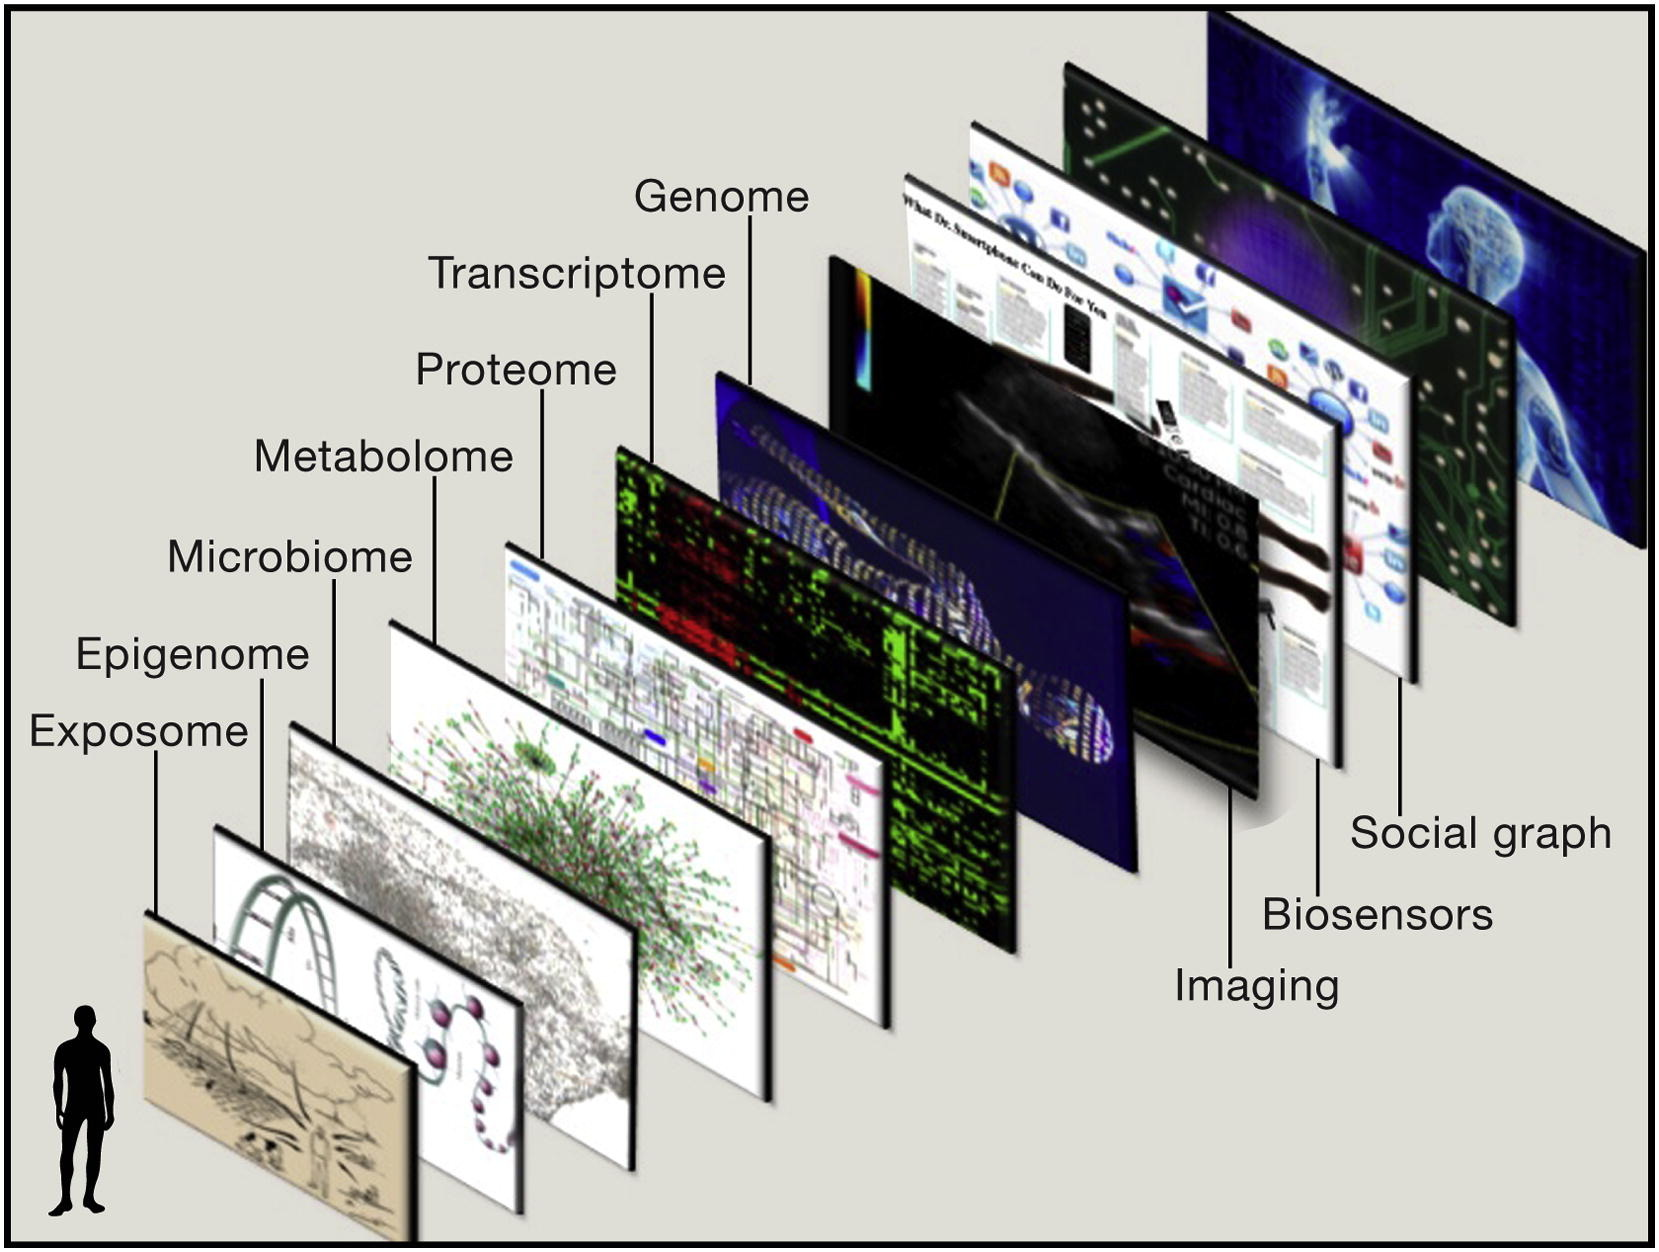
\includegraphics[width=.9\textwidth]{multi-omics2}
\end{figure}

%{\center
%{\scriptsize Source: {\colr \cite{GligPrzulj15}}}
%}
\end{frame}

%%%%%%%%%%%%%%%%%%%%%%%%%%%%%%%%%%%%%%%%%%%%%%%%%%%%%%%%%%%%%%%
\begin{frame}

\begin{figure}
\centering
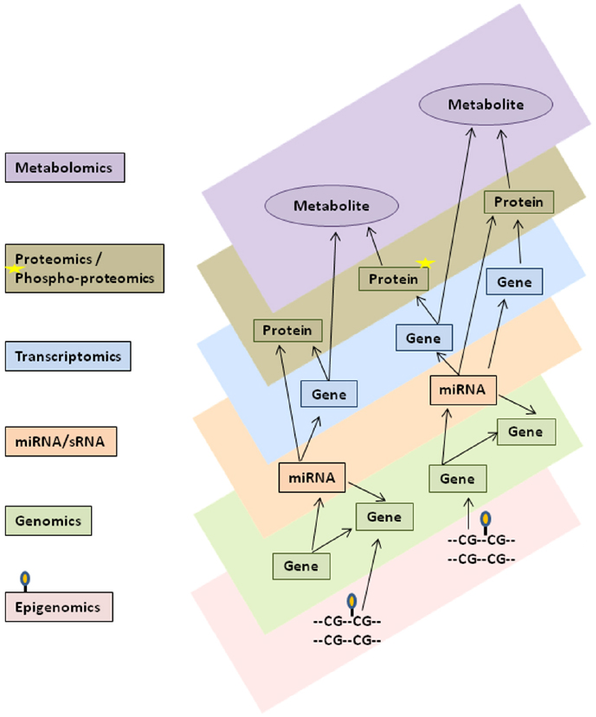
\includegraphics[height=.9\textheight]{multi-omics}
\end{figure}

%{\center
%{\scriptsize Source: {\colr \cite{GligPrzulj15}}}
%}
\end{frame}

%%%%%%%%%%%%%%%%%%%%%%%%%%%%%%%%%%%%%%%%%%%%%%%%%%%%%%%%%%%%%%%
\begin{frame}
\frametitle{Summary}

These connections can be different inside different organs, experimental conditions, or for different subtypes of the same disease;

\begin{center}
\begin{scriptsize}
\begin{tabular}{ccc}
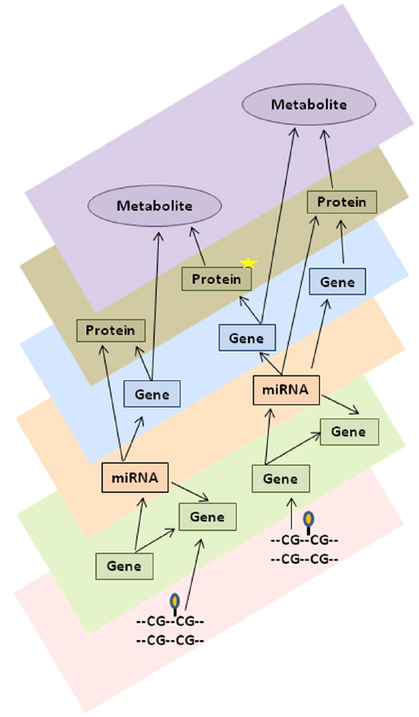
\includegraphics[width=.2\textwidth]{multi-omics1}
\vspace{.5em}
& 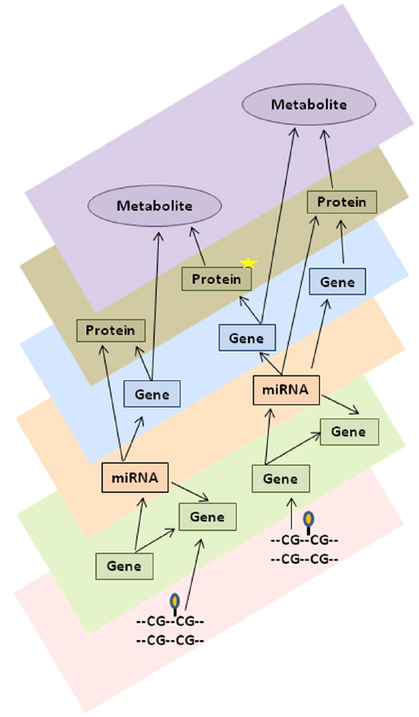
\includegraphics[width=.2\textwidth]{multi-omics1}
\vspace{.5em}
& 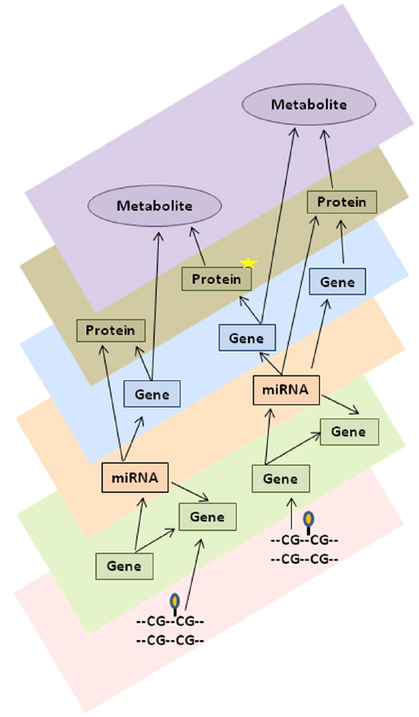
\includegraphics[width=.2\textwidth]{multi-omics1}
\vspace{.5em}\\
Liver & Kidney & Lungs\\

\includegraphics[width=.2\textwidth]{liver}
\vspace{.5em}
& 
\includegraphics[width=.2\textwidth]{kidney}
\vspace{.5em}
& 
\includegraphics[width=.2\textwidth]{lungs}
\vspace{.5em}
\end{tabular}
\end{scriptsize}
\end{center}
\end{frame}
%%%%%%%%%%%%%%%%%%%%%%%%%%%%%%%%%%%%%%%%%%%%%%%%%%%%%%%%%%%%%%%

\begin{frame}
\frametitle{Connection to precision medicine}

\begin{figure}
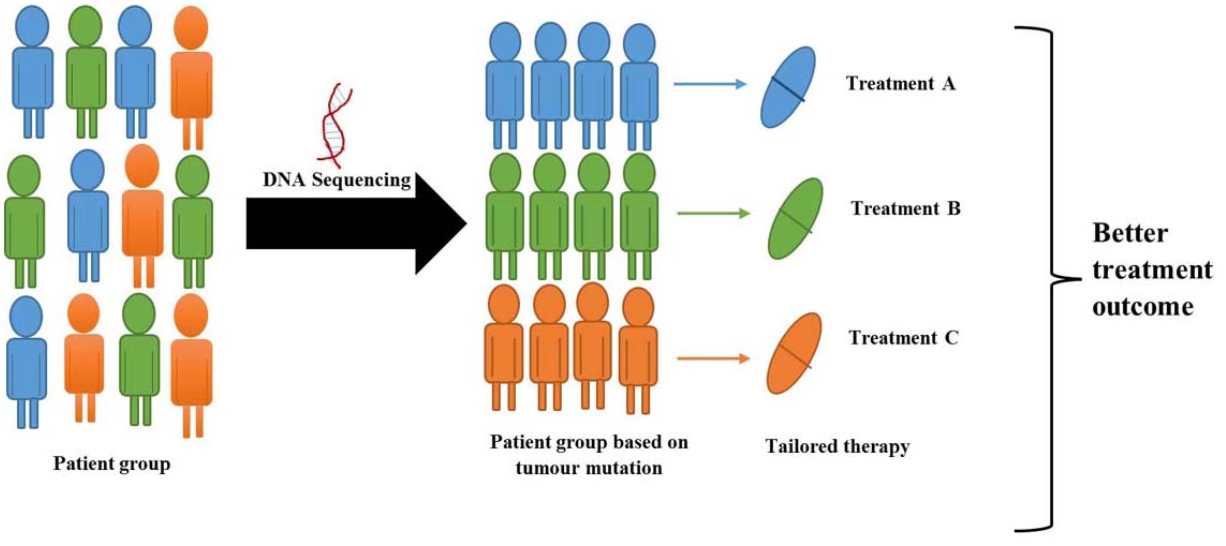
\includegraphics[width=.9\textwidth]{precision-medicine}
\end{figure}

\end{frame}
%%%%%%%%%%%%%%%%%%%%%%%%%%%%%%%%%%%%%%%%%%%%%%%%%%%%%%%%%%%%%%%

\begin{frame}
\frametitle{Connection to precision medicine}
The connections between layers can be different for different patient profiles.

\begin{center}
\begin{scriptsize}
\begin{tabular}{ccc}
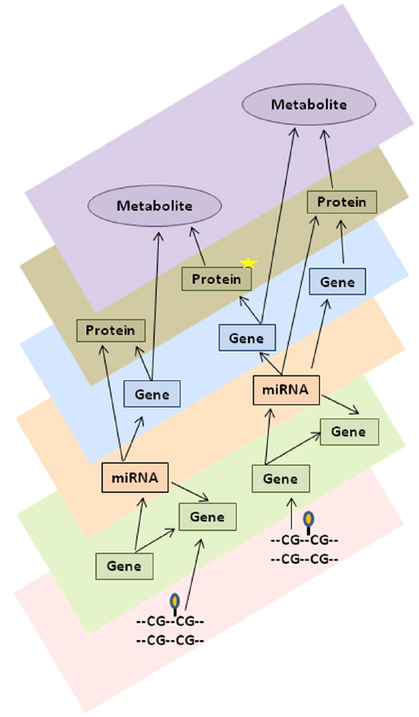
\includegraphics[width=.2\textwidth]{multi-omics1}
\vspace{.5em}
& 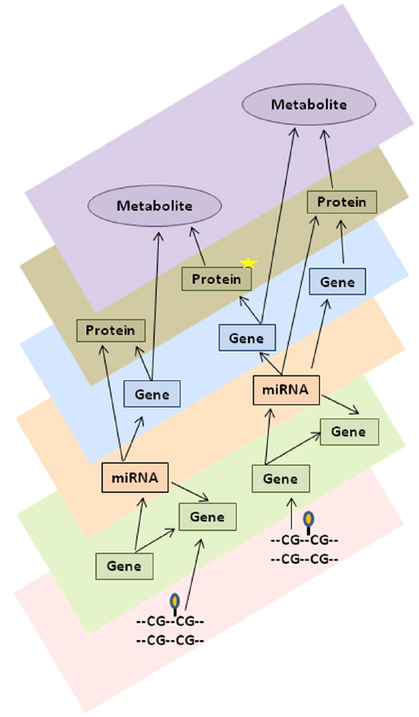
\includegraphics[width=.2\textwidth]{multi-omics1}
\vspace{.5em}
& 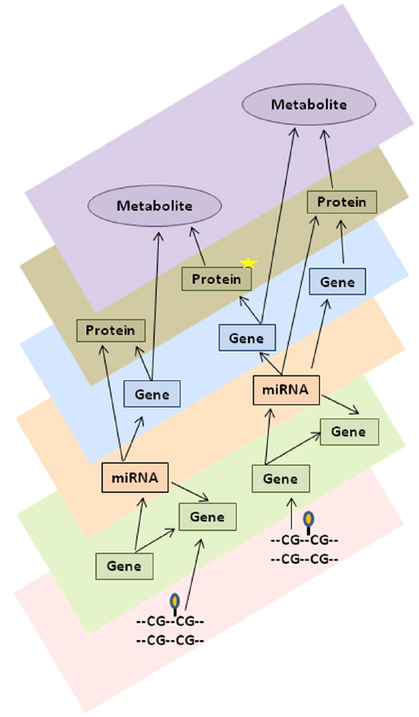
\includegraphics[width=.2\textwidth]{multi-omics1}
\vspace{.5em}\\
Treatment 1 & Treatment 2 & Treatment 3\\
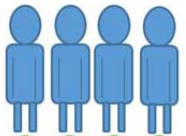
\includegraphics[width=.2\textwidth]{profile1}
\vspace{.5em}
& 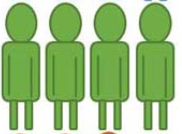
\includegraphics[width=.2\textwidth]{profile2}
\vspace{.5em}
& 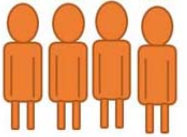
\includegraphics[width=.2\textwidth]{profile3}
\vspace{.5em}
\end{tabular}
\end{scriptsize}
\end{center}
\end{frame}
%%%%%%%%%%%%%%%%%%%%%%%%%%%%%%%%%%%%%%%%%%%%%%%%%%%%%%%%%%%%%%%

\begin{frame}
\frametitle{What we do}

{\colrbf Statistical inference for hierarchical graphical models.}
\vspace{1em}

In this work we propose a general statistical framework based on graphical models for {\colbit horizontal} (i.e. across conditions or subtypes) {\colbit and vertical} (i.e. across different layers containing data on molecular compartments) {\colbit integration of information} in data from such complex biological structures.

\vspace{1em}
Specifically, we perform {\colbit joint estimation and hypothesis testing} for all the connections in these structures.

\end{frame}

%%%%%%%%%%%%%%%%%%%%%%%%%%%%%%%%%%%%%%%%%%%%%%%%%%%%%%%%%%%%%%%%
\frame{\frametitle{Table of contents}\tableofcontents}
%%%%%%%%%%%%%%%%%%%%%%%%%%%%%%%%%%%%%%%%%%%%%%%%%%%%%%%%%%%%%%%%

%%%%%%%%%%%%%%%%%%%%%%%%%%%%%%%%%%%%%%%%%%%%%%%%%%%%%%%%%%%%%%%%
\section{Multiple multi-level graphical models}
%%%%%%%%%%%%%%%%%%%%%%%%%%%%%%%%%%%%%%%%%%%%%%%%%%%%%%%%%%%%%%%%

\begin{frame}
\frametitle{Gaussian Graphical models}

$$
\BX = (X_1, \ldots, X_p)^T \sim \cN_p (0, \Sigma_x)
$$
%
Non-zero entries in the {\colb precision matrix} $\Omega_x = \Sigma_x^{-1}$ gives edges of the network.

\begin{figure}
\centering
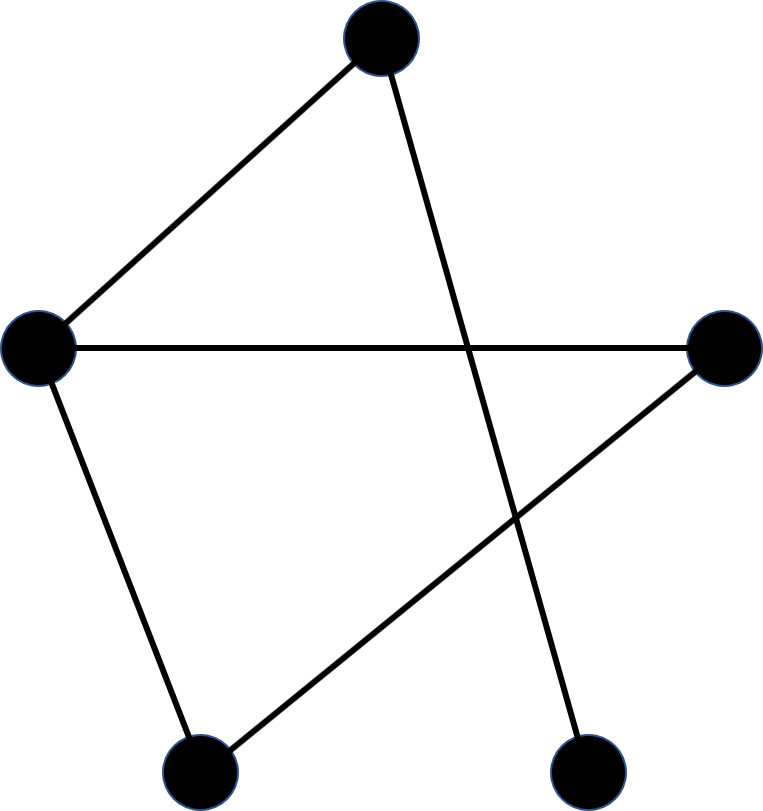
\includegraphics[width=.4\textwidth]{formulation_2}
\end{figure}

Sparse estimation of $\Omega_x$: {\colr \cite{MeisenBuhlmann06}}

Multiple testing and error control: {\colr \cite{DrtonPerlman07}}.

\end{frame}
%%%%%%%%%%%%%%%%%%%%%%%%%%%%%%%%%%%%%%%%%%%%%%%%%%%%%%%%%%%%%%%%

\begin{frame}
\frametitle{Multiple Gaussian Graphical models}

\begin{align*}
& \BX^k = (X_1^k, \ldots, X_p^k)^T \sim \cN_p (0, \Sigma_x^k); \quad
\Omega_x^k = (\Sigma_x^k)^{-1}\\
& k = 1, 2, \ldots, K
\end{align*}

\begin{figure}
\centering
\begin{tabular}{ccc}
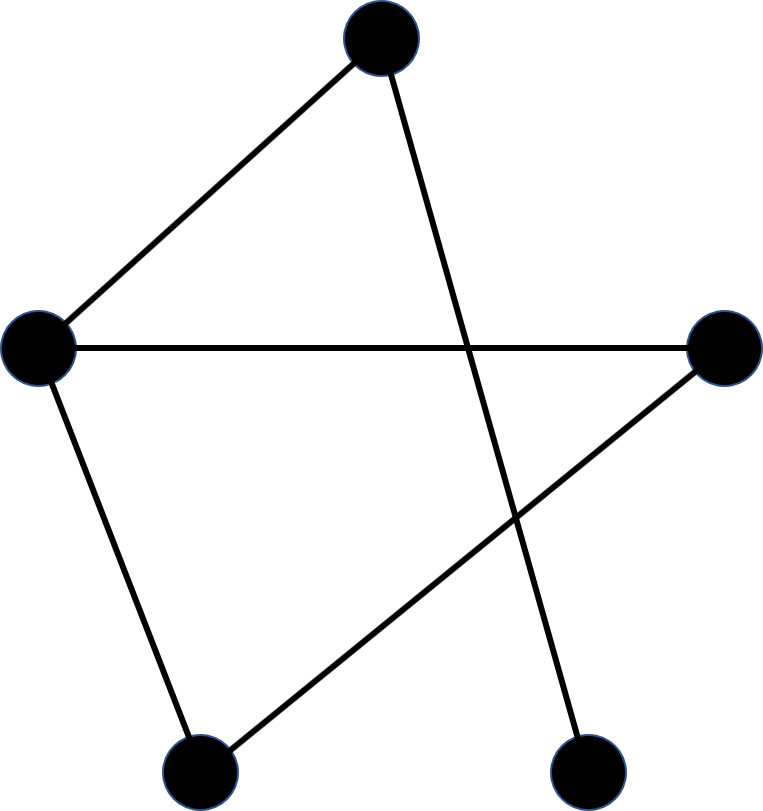
\includegraphics[width=.25\textwidth]{formulation_2} & 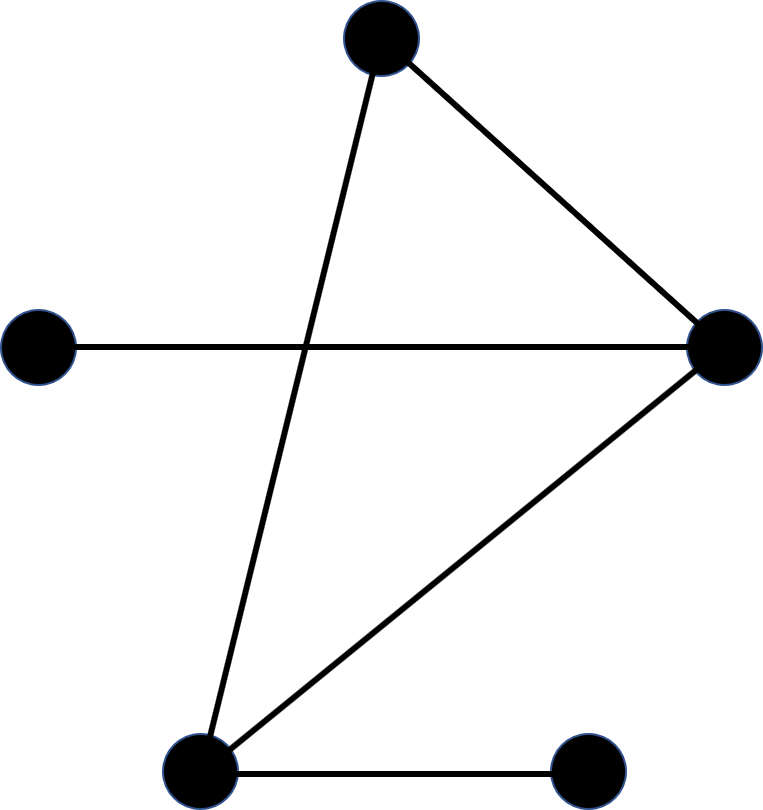
\includegraphics[width=.25\textwidth]{formulation_3}
& 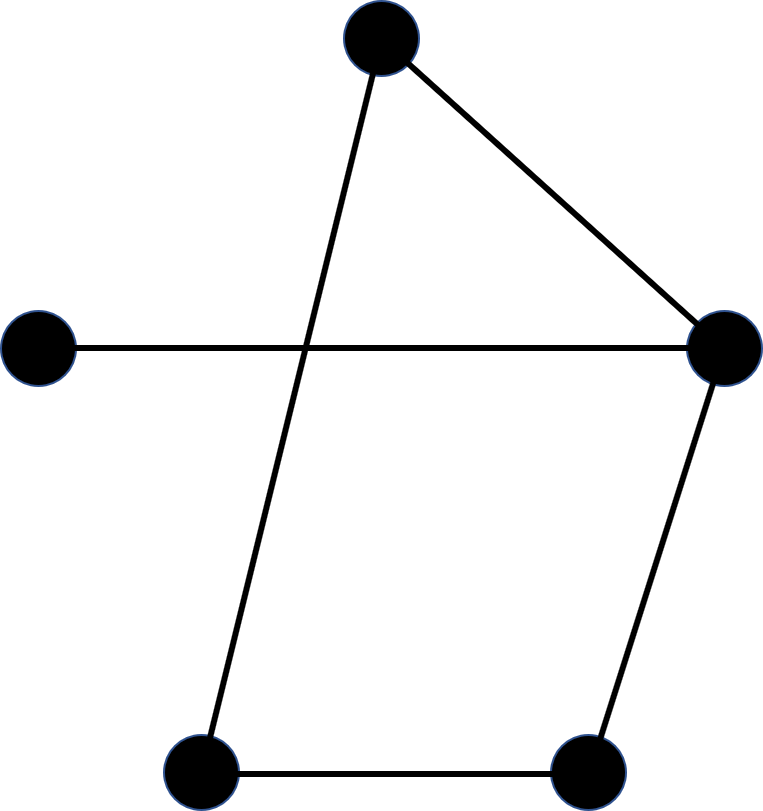
\includegraphics[width=.25\textwidth]{formulation_4}
\\
$k=1$ & $k=2$ & $k=3$
\end{tabular}
\hspace{1em}
\end{figure}
\vspace{1em}

\begin{itemize}
\item Joint estimation of $\{ \Omega_x^k \}$: {\colr \cite{GuoEtal11, MaMichailidis15}}
\vspace{1em}

\item Difference and similarity testing with FDR control: {\colr\cite{Liu17}}
\end{itemize}
\end{frame}
%%%%%%%%%%%%%%%%%%%%%%%%%%%%%%%%%%%%%%%%%%%%%%%%%%%%%%%%%%%%%%%%

\begin{frame}
\frametitle{Multi-Layered Gaussian Graphical models}

\begin{minipage}{.49\textwidth}
%
\onslide<2->{
{\color{black}
\begin{align*}
& \BE = (E_1, \ldots, E_q)^T \sim \cN_q (0, \Sigma_y);\\
& \BF = (F_1, \ldots, F_r)^T \sim \cN_r (0, \Sigma_z);\\
& \Omega_y = (\Sigma_y)^{-1}, \Omega_z = (\Sigma_z)^{-1}\\
& \BY = \BX^T \bfB + \BE,\\
& \BZ = \BY^T \bfC + \BF.\\
\end{align*}}
%

\vspace{-3em}
\begin{itemize}
\item $\Omega_x, \Omega_y, \Omega_z$ give undirected within-layer edges, while $\bfB, \bfC$ gives directed between-layer edges.
\vspace{1em}
}

\onslide<3>{
\item Sparse estimation of the components: {\colr\cite{LinEtal16}}.

\item Testing: {\colrbf ??}
}
\end{itemize}
\end{minipage}
%
\begin{minipage}{.49\textwidth}
\centering
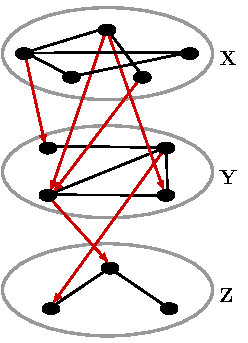
\includegraphics[height=.7\textheight]{multilayer.pdf}
\end{minipage}

\end{frame}
%%%%%%%%%%%%%%%%%%%%%%%%%%%%%%%%%%%%%%%%%%%%%%%%%%%%%%%%%%%%%%%%

\begin{frame}
\frametitle{Multiple Multi-layered Gaussian Graphical models}

\begin{tabular}{c}
\includegraphics[width=.9\textwidth]{multi2layer}
\end{tabular}

%
\onslide<2>{
\begin{align*}
& \BE^k = (E_1^k, \ldots, E_q^k)^T \sim \cN_q (0, \Sigma_y^k); \quad
\Omega_y^k = (\Sigma_y^k)^{-1}\\
& \BF^k = (F_1^k, \ldots, F_r^k)^T \sim \cN_r (0, \Sigma_z^k); \quad
\Omega_y^k = (\Sigma_y^k)^{-1}\\
& \BY^k = (\BX^k)^T \bfB^k + \BE^k,\\
& \BZ^k = (\BY^k)^T \bfC^k + \BF^k; \quad k = 1, 2, \ldots, K
\end{align*}
%
}
\end{frame}
%%%%%%%%%%%%%%%%%%%%%%%%%%%%%%%%%%%%%%%%%%%%%%%%%%%%%%%%%%%%%%%%

\begin{frame} %% one-by-one appear
\frametitle{What we do}

\begin{outline}
\onslide<2->{ \1 We decompose the multi-layer problem into a series of two layer problems.}

\vspace{1em}
\onslide<3->{
\1 We estimate $\{ \Omega_x^k, \Omega_y^k, \bfB^k \}$ jointly for all $k$ from a single model;}
\onslide<4->{
\2 Incorporate structural informartion using group sparsity,}
\onslide<5->{
\2 Propose algorithm to compute solutions, derive their convergence properties.}

\vspace{1em}
\onslide<6->{
\1 Devise a full pairwise testing procedure for rows of $\bfB^k$;}

\onslide<7->{
\2 For $K=2$, propose a test for row-wise differences $\bfb_i^1 - \bfb_i^2$;}

\onslide<8->{
\2 Perform multiple testing for elementwise differences $b_{ij}^1 = b_{ij}^2, j = 1, 2, \ldots, q$ within a row.}

\vspace{1em}
\onslide<11>{
\1 Use simulations for performance evaluation.}
\end{outline}
\end{frame}
%%%%%%%%%%%%%%%%%%%%%%%%%%%%%%%%%%%%%%%%%%%%%%%%%%%%%%%%%%%%%%%%

\section{Preliminaries}
%%%%%%%%%%%%%%%%%%%%%%%%%%%%%%%%%%%%%%%%%%%%%%%%%%%%%%%%%%%%%%%%

\begin{frame}
\frametitle{Preliminaries}

\visible<2->{
\begin{itemize}
\item $\cY = \{ \bfY^1, \ldots, \bfY^K\}, \cX = \{ \bfX^1, \ldots, \bfX^K\}$;

\item ${\colg \Omega_x = \{ \Omega_x^1, \ldots, \Omega_x^K \}}, {\colb \Omega_y = \{ \Omega_y^1, \ldots, \Omega_y^K \}},
{\colr \cB = \{ \bfB^1, \ldots, \bfB^K \}}$;
\end{itemize}
}

\visible<3->{
\begin{block}{}
{\bf Linear model}: $\bfy = \bfX \bfbeta + \bfepsilon$, with $\bfX \in \BR^{n \times p}, \bfbeta \in \BR^p, \bfepsilon \sim \cN({\bf 0}, \sigma^2 \bfI)$ with $\sigma >0$;

\vspace{1em}
{\bf Lasso:} $\widehat \bfbeta = \argmin_\bfbeta \| \bfy - \bfX \bfbeta \|^2/n + \lambda \| \bfbeta \|_1$;

\visible<4>{
\vspace{1em}
{\bf Group lasso:}
%
$$
\widehat \bfbeta = \argmin_\bfbeta \frac{1}{n} \| \bfy - \bfX \bfbeta \|^2 + \lambda \sum_{g \in \cG} \| \bfbeta_g \|
$$
%
where $\cG$ is a {\it partition} of $\{1, 2, \ldots, p \}$.

\vspace{1em}
{\colb Example: $p=7, \cG = \{ [1,2], [3,4],[5,6,7] \}$. Then
%
$$
\sum_{g \in \cG} \| \bfbeta_g \| = \sqrt{ \beta_1^2 + \beta_2^2} +
\sqrt{ \beta_3^2 + \beta_4^2} +
\sqrt{ \beta_5^2 + \beta_6^2 + \beta_7^2}
$$
}}

\end{block}
}
\end{frame}

%\begin{itemize}
%\item {\bf For single GGM}: Estimate neighboring edges for each node, then refit.
%%
%\begin{align*}
%\widehat \bfzeta_i &= \argmin_{\bfzeta_i} \left\{ \frac{1}{n} \| \bfX_i - \bfX_{-i} \bfzeta_i \|^2 + \nu_n \sum_{i' \neq i} |\zeta_{ii'}| \right\};\\
%\widehat \Omega_x &= \argmin_{\Omega_x \in \cup_i \supp (\bfzeta_i)}
%\{ \Tr (\bfS_x \Omega_x ) + \log \det(\Omega_x) \}
%\end{align*}
%%
%Can do this because $\zeta_{ii'} = -\omega_{ii'}/\omega_{ii}$, so zeros of the precision matrix and neighborhood matrix are same.

%%%%%%%%%%%%%%%%%%%%%%%%%%%%%%%%%%%%%%%%%%%%%%%%%%%%%%%%%%%%%%%%

\section{Joint Multiple Multi-Level Estimation}
%%%%%%%%%%%%%%%%%%%%%%%%%%%%%%%%%%%%%%%%%%%%%%%%%%%%%%%%%%%%%%%%

%%%%%%%%%%%%%%%%%%%%%%%%%%%%%%%%%%%%%%%%%%%%%%%%%%%%%%%%%%%%%%%%

\begin{frame}
\frametitle{Estimation of X-network}

\begin{enumerate} %% break
\onslide<2->{
\item {\colrbf Trick:} Take a node- figure out who its neighbors are. Repeat this for all nodes. This infers the full graph structure.
}

\onslide<3->{
\item {\colbit Estimate neighborhood coefficients} of each X-node, say $\zeta_i = (\bfzeta_i^1, \ldots, \bfzeta_i^K)$ using the group information on the X-network:
%
$$
{\colg \widehat \zeta_i} = \argmin_{\zeta_i} \left\{ \sum_{k=1}^K \frac{1}{n_k} \| \bfX_i^k - \bfX_{-i}^k {\colg \bfzeta_i^k} \|^2 + {\colg \nu_n P(\zeta)} \right\}
$$
}

\onslide<4->{
\item Non-zero supports of $\zeta_i, i = 1,...,p$ give a skeleton set for the corresponding graphs. {\colbit Recover precision matrices} as maximum likelihood estimates over these restricted skeleton sets.} %% break
%
\end{enumerate}

\vspace{1em}

\onslide<5>{
\begin{center} %% break
{\colb Joint Structural Estimation Method (JSEM)}

\cite{MaMichailidis15}
}
\end{center}

\end{frame}

%%%%%%%%%%%%%%%%%%%%%%%%%%%%%%%%%%%%%%%%%%%%%%%%%%%%%%%%%%%%%%%%

\begin{frame}
\frametitle{Estimating XY and Y-networks: the objective function}

\begin{center}
\visible<2->{\includegraphics[width=.9\textwidth]{multitwolayer_j}}
\end{center}

\begin{center}
\begin{tabular}{ccc}%% break
\visible<3->{$ \bfY_j^k$} & \visible<4->{$- \quad \bfE_{-j}^k {\colb  \bftheta_j^k}$} & \visible<5>{$- \quad \bfX^k {\colr \bfB_j^k }$}
\end{tabular}

\visible<4->{$$ \bfE^k = \bfY^k - \bfX^k \bfB^k $$}
\end{center}

\end{frame}
%%%%%%%%%%%%%%%%%%%%%%%%%%%%%%%%%%%%%%%%%%%%%%%%%%%%%

\begin{frame}
\frametitle{The objective function}

\begin{center}
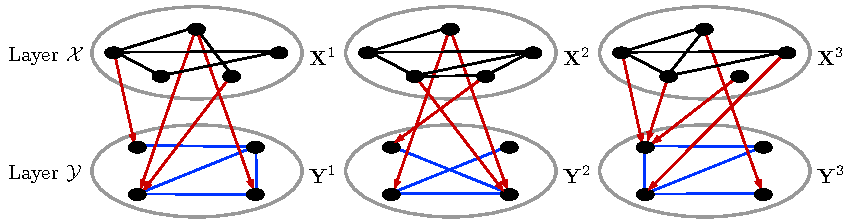
\includegraphics[width=.9\textwidth]{multitwolayer}
\end{center}

\visible<1->{
$$
\sum_{k=1}^K \frac{1}{n_k} \sum_{j=1}^q
\left\| \bfY_j^k - (\bfY_{-j}^k - \bfX^k \bfB_{-j}^k) {\colb  \bftheta_j^k}
- \bfX^k {\colr \bfB_j^k } \right\|^2
$$
}

$$
\visible<2->{ + {\colr \lambda_n \sum_{h \in \cH} \| \bfB^{[h]} \|}}
\visible<3->{ + {\colb \gamma_n \sum_{j' \neq j, g \in \cG_{jj'}} \| \bftheta_{jj'}^{[g]} \|}}
$$
\visible<4>{
\begin{center}
(Ask me what they are later)
\end{center}
}
\end{frame}
%%%%%%%%%%%%%%%%%%%%%%%%%%%%%%%%%%%%%%%%%%%%%%%%%%%%%
%
%\begin{frame}
%\frametitle{Estimation of $\cB, \Omega_y$}
%
%\begin{enumerate} 
%\item Estimate regression coefficient matrices using group information $\cH$:
%\begin{align*}
%\widehat \cB &= \argmin_{\cB} \left\{ \sum_{k=1}^K \frac{1}{n_k}
%\| (\bfY^k - \bfX^k \bfB^k) \widehat \bfT^k \|_F^2 + 
%\lambda_n \sum_{h \in \cH} \| \bfB^{[h]} \| \right\}
%\end{align*}
%%
%where $\widehat t_{jj}^k = 1, \widehat t_{jj'}^k = - \widehat \theta_{jj'}^k$.
%
%\item Estimate neighborhood coefficients of each Y-node, say $\Theta_j = (\bftheta_j^1, \ldots, \bftheta_j^K)$ using the group sparsity information $\cG_y$:
%%
%$$
%\widehat \Theta_j = \argmin_{\Theta_j} \left\{ \sum_{k=1}^K \frac{1}{n_k} \| \widehat \bfE_j^k - \widehat \bfE_{-j}^k \bftheta_j^k \|^2 + \gamma_n \sum_{j' \neq j, g \in \cG_{y,jj'}} \| \bftheta_{jj'}^{[g]} \| \right\}
%$$
%%% break
%
%%% break
%\item Estimate precision matrices as MLE over the restricted supports: %% break
%%
%\begin{align*}
%\widehat E_y^k &= \{(j,j'): 1 \leq j < j' \leq q, \widehat \theta_{jj'}^k \neq 0 \text{ OR } \widehat \theta_{j'j}^k \neq 0 \},\\
%\widehat \Omega_y^k &= \argmin_{\Omega_y^k \in \BS_+ (\widehat E_y^k)}
%\left\{ \Tr (\widehat \bfS_y^k \Omega_y^k ) - \log \det (\Omega_y^k) \right\}.
%\end{align*}
%%
%\end{enumerate}
%
%
%\end{frame}

%%%%%%%%%%%%%%%%%%%%%%%%%%%%%%%%%%%%%%%%%%%%%%%%%%%%%%%%%%%%%%%%

\begin{frame}
\frametitle{The estimator}

\begin{center}
{\colrbf Joint Multiple Multi-Level Estimation (JMMLE)}
\end{center}

\begin{enumerate}
\visible<2->{
\item Solve for $\{ \cB, \Theta\}$:
%
\begin{align*}
\{ \widehat \cB, \widehat \Theta \} &=
\argmin_{\cB, \Theta} \left\{ \sum_{k=1}^K \frac{1}{n_k} \sum_{j=1}^q
\left\| \bfY_j^k - ( \bfY_{-j}^k - \bfX^k \bfB_{-j}^k) {\colb \bftheta_j^k}
- \bfX^k {\colr \bfB_j^k} \right\|^2 \right.\\
& + {\colr \lambda_n \sum_{h \in \cH} \| \bfB^{[h]}} \|
\left. + {\colb \gamma_n  \sum_{j' \neq j, g \in \cG_{jj'}} \| \bftheta_{jj'}^{[g]} \|} \right\}
\end{align*}
}
%% break
\visible<3>{
\item Recover Y-precision matrices as MLE over the Y-network skeleton sets
}
\end{enumerate}

\end{frame}
%%%%%%%%%%%%%%%%%%%%%%%%%%%%%%%%%%%%%%%%%%%%%%%%%%%%%%%%%%%%%%%%
\begin{frame}
\frametitle{Computational algorithm}
\begin{align*}
\{ \widehat \cB, \widehat \Theta \} &= \argmin_{\cB, \Theta}
\left\{ f(\cY, \cX, {\colr \cB}, {\colb \Theta}) + {\colr P(\cB)} + {\colb Q(\Theta)} \right\}
\end{align*}

The objective function is biconvex, so we solve the above by the following alternating iterative algorithm:

\begin{enumerate}
\item Start with initial estimates of $\cB$ and $\Theta$, say $\cB^{(0)}, \Theta^{(0)}$.
\item Iterate:
%
\begin{align*}
\cB^{(t+1)} &= \argmin_\cB \left\{ f ( \cY, \cX, {\colr \cB}, \Theta^{(t)}) + {\colr Q (\cB)} \right\}\\
\Theta^{(t+1)} &= \argmin_\Theta \left\{ f ( \cY, \cX, \cB^{(t+1)}, {\colb \Theta}) + {\colb P (\Theta)} \right\}
\end{align*}
\item Continue till convergence.
\end{enumerate}
\end{frame}
%%%%%%%%%%%%%%%%%%%%%%%%%%%%%%%%%%%%%%%%%%%%%%%%%%%%%%%%%%%%%%%%
%
%\begin{frame}
%\frametitle{The two subproblems}
%\begin{align*}
%\widehat \cB &=
%\argmin_{\cB} \left\{
%\sum_{k=K}^q \frac{1}{n_k} \sum_{j=1}^q
%\left\| \bfY_j^k - ( \bfY_{-j}^k - \bfX^k {\colr \bfB_{-j}^k} ) \widehat \bftheta_j^k
%- \bfX^k {\colr \bfB_j^k} \right\|^2
%+ {\colr \lambda_n \sum_{h \in \cH} \| \bfB^{[h]} \|} \right\}\\
%&= \argmin_{\cB} \left\{ \sum_{k=1}^K \frac{1}{n_k}
%\| (\bfY^k - \bfX^k {\colr \bfB^k}) \widehat \bfT^k \|_F^2 +
%+ {\colr \lambda_n \sum_{h \in \cH} \| \bfB^{[h]} \|} \right\}
%\end{align*}
%%
%where $\widehat t_{jj}^k = 1, \widehat t_{jj'}^k = - \widehat \theta_{jj'}^k$.
%
%\begin{align*}
%\widehat \Theta &=
%\argmin_{\Theta} \left\{ \sum_{k=K}^q \frac{1}{n_k} \sum_{j=1}^q
%\left\| \bfY_j^k - ( \bfY_{-j}^k - \bfX^k \widehat \bfB_{-j}^k) {\colb \bftheta_j^k}
%- \bfX^k \widehat \bfB_j^k \right\|^2 
%+ {\colb \gamma_n \sum_{j' \neq j, g \in \cG_{jj'}} \| \bftheta_{jj'}^{[g]} \|} \right\}\\
%&= \argmin_{\Theta} \left\{ 
%\sum_{k=K}^q \frac{1}{n_k} \sum_{j=1}^q
%\| \widehat \bfE_j^k - \widehat \bfE_{-j}^k {\colb \bftheta_j^k} \|^2
%+ {\colb \gamma_n \sum_{j' \neq j, g \in \cG_{jj'}} \| \bftheta_{jj'}^{[g]} \|} \right\}
%\end{align*}
%%
%where $\widehat \bfE^k = \bfY^k - \bfX^k \widehat \bfB^k$.
%
%\end{frame}
%
%%%%%%%%%%%%%%%%%%%%%%%%%%%%%%%%%%%%%%%%%%%%%%%%%%%%%%%%%%%%%%%%

\begin{frame}
\frametitle{Non-asymptotic error bounds for $\widehat \cB$}

For $\lambda_n \geq 4 \sqrt{| h_{\max} |} \BR_0 {\colr \sqrt{ \frac{ \log(pq)}{n}}}$, the following hold with probability approaching 1 as $n \rightarrow \infty$,
%
\begin{align*}
\| \widehat \bfbeta - \bfbeta_0 \|_1 & \leq \frac{48 \sqrt{ | h_{\max} |} {\colr s_\beta \lambda_n}}{ \psi^*} \\
\| \widehat \bfbeta - \bfbeta_0 \| & \leq \frac{12 {\colr \sqrt s_\beta \lambda_n}}{ \psi^*} \\
\sum_{h \in \cH} \| \bfbeta^{[h]} - \bfbeta_0^{[h]} \| & \leq \frac{48 {\colr s_\beta \lambda_n}}{ \psi^*}
\end{align*}
%
with $\psi^*, \BR_0$ being constants, and $\bfbeta = (\ve(\bfB^1)^T, \ldots, \ve(\bfB^K)^T)^T$, $| h_{\max} |$ the maximum group size in $\bfbeta_0$ (the true $\bfbeta$) and $s_\beta$ the sparsity of $\bfbeta_0$.
\end{frame}

%%%%%%%%%%%%%%%%%%%%%%%%%%%%%%%%%%%%%%%%%%%%%%%%%%%%%%%%%%%%%%%%

\begin{frame}
\frametitle{Error bounds for $\widehat \Theta, \widehat\Omega$}

For $\gamma_n = 4 \sqrt{| g_{\max}|} \BQ_0 {\colb \sqrt{ \frac{ \log(pq)}{n}}}$, the following hold with probability approaching 1 as $n \rightarrow \infty$,
%
\begin{align*}
\| \widehat \Theta_j - \Theta_{0,j} \|_F & \leq \frac{12 {\colb \sqrt{s_j} \gamma_n}}{\psi} \\
\sum_{j \neq j', g \in \cG_y^{jj'}} \| \widehat \bftheta_{jj'}^{[g]} - \bftheta_{0,jj'}^{[g]} \| & \leq \frac{48 {\colb s_j \gamma_n}}{\psi} \\
%\left| \supp (\widehat \Theta_j) \right| & \leq \frac{128 s_j}{ \psi}\\
\frac{1}{K} \sum_{k=1}^K \| \widehat \Omega_y^k - \Omega_y^k \|_F & \leq
O \left( \frac{{\colb \sqrt S \gamma_n }}{\sqrt K} \right)\\
\end{align*}
%
with $\psi, \BQ_0$ being constants, $| g_{\max} |$ the maximum group size in $\Theta_0$, $s_j$ the sparsity of $\Theta_j$ and $S = \sum_j s_j$.
\end{frame}

%%%%%%%%%%%%%%%%%%%%%%%%%%%%%%%%%%%%%%%%%%%%%%%%%%%%%%%%%%%%%%%%
\section{Hypothesis testing in multi-layer models}
%%%%%%%%%%%%%%%%%%%%%%%%%%%%%%%%%%%%%%%%%%%%%%%%%%%%%%%%%%%%%%%%

\begin{frame}
\frametitle{Motivation}

\begin{itemize}
\onslide<2->{
\item Find out if an upper layer variable has a significant downstream effects, {\colb e.g. if a gene influences the activity of {\it any} protein.}
\vspace{1em}
}

\onslide<3->{
\item How does this downstream effect vary across different horizontal category, {\colb e.g. gene has downstream effect on patient profile 1 but not on profile 2.}
\vspace{1em}
}

\onslide<4>{
\item Which of the downstream effects are significant? How do they differ across subtypes? {\colb e.g. which exact proteins does the gene affect for each patient profile}
}
\end{itemize}

\end{frame}
%%%%%%%%%%%%%%%%%%%%%%%%%%%%%%%%%%%%%%%%%%%%%%%%%%%%%%%%%%%%%%%%

\begin{frame}
\frametitle{High-dimensional hypothesis testing}

\begin{block}{Debiased estimators (Zhang and Zhang, 2014)}
\begin{itemize}
\visible<2->{
\item Lasso: $\widehat \bfbeta = \argmin_\bfbeta \| \bfy - \bfX \bfbeta \|^2/n + \lambda \| \bfbeta \|_1$;
}

\visible<3->{
\item Debiased estimator:
%
$$
\hat \beta_j^{(\text{deb})} = \hat \beta_j + \frac{\bfz_j^T ( \bfy - \bfX \widehat \bfbeta)}{\bfz^T \bfx_j},
$$
%
where $\bfz_j$ is the vector of residuals from the $\ell_1$-penalized regression of $\bfx_j$ on $\bfX_{-j}$.
}
\visible<4->{
\item Asymptotic normal distribution:
%
$$
\frac{\hat \beta_j^{(\text{deb})} - \beta_j^0}{\| \bfz_j \|/| \bfz_j^T \bfx_j |} \sim N(0, \sigma^2)
$$
%
}
\end{itemize}

\end{block}

\visible<5>{
The debiasing factor for the $j^{\Th}$ coefficient is obtained by taking residuals from the regularized regression and scale them using the { \colbit projection of $\bfx_j$ onto a space approximately orthogonal to it}.
}
\end{frame}
%%%%%%%%%%%%%%%%%%%%%%%%%%%%%%%%%%%%%%%%%%%%%%%%%%%%%%%%%%%%%%%%

\begin{frame}
\frametitle{What we do}
\begin{itemize}
%% break
\onslide<2->{
\item  We propose a {\colb debiased estimator} for $\bfb_i^k$ that makes use of already computed model quantities, and establish asymptotic properties of its scaled version,
}
%% break
\onslide<3->{
\vspace{1em}
\item We assume $K = 2$, and propose an {\colb asymptotic test} for detecting differential effects of a variable in the upper layer, i.e. testing for the null hypothesis $H_0 : \bfb^1_{0i} = \bfb^2_{0i}$,
}
%% break
\onslide<4>{
\vspace{1em}
\item We also propose {\colb pairwise simultaneous tests} with False Discovery Rate (FDR) control across $j = 1, \ldots, q$ for detecting the elementwise differences $b_{0ij}^1 = b_{0ij}^2$.
}
\end{itemize}

\end{frame}
%%%%%%%%%%%%%%%%%%%%%%%%%%%%%%%%%%%%%%%%%%%%%%%%%%%%%%%%%%%%%%%%

%%%%%%%%%%%%%%%%%%%%%%%%%%%%%%%%%%%%%%%%%%%%%%%%%%%%%%%%%%%%%%%%
\section{Numerical experiments}
%%%%%%%%%%%%%%%%%%%%%%%%%%%%%%%%%%%%%%%%%%%%%%%%%%%%%%%%%%%%%%%%

\begin{frame}
\frametitle{Simulation setup}
\begin{itemize}
\item Number of categories ($K$) = 5;

\item Structured $\{ \Omega_x\}, \{\Omega_y\}, \cB$;

\item Groups in $\cB,\Omega_x$ are non-zero with probability $5/p$, and their elements come from Unif$[-1, -0.5] \cup [0.5,1]$;

\item Groups in $\Omega_y$ are non-zero with probability $5/q$, and their elements come from Unif$[-1, -0.5] \cup [0.5,1]$;

\item We generate size-$n$ i.i.d. samples $\bfX^k$ from $\cN_p(0, \Sigma_x^k)$, and $\bfE^k$ from $\cN_p(0, \Sigma_y^k)$, then obtain $\bfY^k = \bfX^k \bfB^k + \bfE^k$;

\item 50 Replications.

\item Tuning parameters:
$$
\gamma_n \in \left\{ 0.3, 0.4, ..., 1 \right\} \sqrt{\frac{\log q}{n}}, 
\lambda_n \in \left\{ 0.4, 0.6, ..., 1.8 \right\} \sqrt{\frac{\log p}{n}}
$$

\end{itemize}
\end{frame}
%%%%%%%%%%%%%%%%%%%%%%%%%%%%%%%%%%%%%%%%%%%%%%%%%%%%%%%%%%%%%%%%

\begin{frame}
\frametitle{Evaluation metrics}
\begin{enumerate}
\item True positive Rate-
%
\[
\text{TPR} (\widehat \cB) = \frac{1}{K} \sum_{k=1}^K \frac{ | \supp(\widehat \bfB^k) \cup \supp (\bfB_0^k)|}{ | \supp (\bfB_0^k)| }
\]
\item True negatives-
%
\[
\text{TNR} (\widehat \cB) = \frac{1}{K} \sum_{k=1}^K \frac{ | \supp^c(\widehat \bfB^k) \cup \supp^c (\bfB_0^k)|}{ | \supp^c (\bfB_0^k)| }
\]
%
\item Relative error in Frobenius norm-
%
\[
\text{RF} (\widehat \cB) = \frac{1}{K} \sum_{k=1}^K \frac{\| \widehat \bfB^k - \bfB_0^k \|_F}{\| \bfB_0^k \|_F}
\]
%

\item Matthews correlation coefficient (MCC).
\end{enumerate}

Same metrics are used for $\widehat \Theta$.
\end{frame}
%%%%%%%%%%%%%%%%%%%%%%%%%%%%%%%%%%%%%%%%%%%%%%%%%%%%%%%%%%%%%%%%
\begin{frame}
\frametitle{Results}

\begin{scriptsize}
\begin{tabular}{ccccccc}
\hline
    $(\pi_x, \pi_y)$ & $(p,q,n)$   & Method   & TPR            & TNR            & MCC & RF            \\ \hline
    $(5/p, 5/q)$   & (60,30,100)   & JMMLE    & \textbf{0.97(0.02)}  & 0.99(0.003)  & \textbf{0.96(0.014)} & 0.24(0.033) \\
    ~              & ~             & Separate & 0.96(0.018) & 0.99(0.004)  & 0.93(0.014) & 0.22(0.029) \\\cline{2-7}
    %
    ~              & (30,60,100)   & JMMLE    & 0.97(0.013) & 0.99(0.002)  & \textbf{0.96(0.008)} & 0.27(0.024) \\
    ~              & ~             & Separate & 0.99(0.009) & 0.99(0.003)  & 0.93(0.017) & 0.18(0.021) \\\cline{2-7}
    %
    ~              & (200,200,150) & JMMLE    & 0.98(0.011) & \textbf{1.0(0) }      & \textbf{0.99(0.005)} & \textbf{0.16(0.025)} \\
    ~              & ~             & Separate & 0.99(0.001) & 0.99 (0.001) & 0.88(0.009) & 0.18(0.007) \\\cline{2-7}
    %
    ~              & (300,300,150) & JMMLE    & \textbf{1.0(0.001)}  & \textbf{1.0(0)}       & \textbf{0.99(0.001)} & \textbf{0.14 (0.015)}\\
    ~              & ~             & Separate & 1.0(0.001)  & 0.99(0.001)  & 0.84(0.01)  & 0.21(0.007)\\\hline
    %
    $(30/p, 30/q)$ & (200,200,100) & JMMLE    & \textbf{0.97(0.017)} & \textbf{1.0(0)}       & \textbf{0.98(0.008)} & \textbf{0.21(0.032)} \\
    ~              & ~             & Separate & 0.32(0.01)  & 0.99(0.001)  & 0.49(0.009) & 0.85(0.06)  \\\cline{2-7}
    %
    ~              & (200,200,200) & JMMLE    & \textbf{0.99(0.006)} & \textbf{1.0(0)}       & \textbf{0.99(0.007)} & \textbf{0.13(0.016)} \\
    ~              & ~             & Separate & 0.97(0.004) & 0.98(0.001)  & 0.93(0.002) & 0.19(0.07)  \\    \hline
\end{tabular}

\begin{center}
Table of outputs for estimation of regression matrices, giving empirical mean and standard deviation (in brackets) of each evaluation metric over 50 replications.
\end{center}
\end{scriptsize}

\end{frame}
%%%%%%%%%%%%%%%%%%%%%%%%%%%%%%%%%%%%%%%%%%%%%%%%%%%%%%%%%%%%%%%%

\begin{frame}
\frametitle{Results}

\begin{scriptsize}
\begin{tabular}{ccccccc}
    \hline
    $(\pi_x, \pi_y)$ & $(p,q,n)$   & Method   & TPR            & TNR             & MCC & RF            \\ \hline
    $(5/p, 5/q)$   & (60,30,100)   & JMMLE    & 0.76(0.018) & 0.90(0.006)  & \textbf{0.61(0.024)}  & \textbf{0.32(0.008)} \\
    ~              & ~             & Separate & 0.77(0.031) & 0.92(0.007)  & 0.56(0.03)   & 0.51(0.017) \\
    ~              & ~             & JSEM     & 0.24(0.013) & 0.8(0.003)   & 0.05(0.015)  & 1.03(0.002)\\\cline{2-7}
    %
    ~              & (30,60,100)   & JMMLE    & 0.7(0.018)  & \textbf{0.94(0.002)}  & 0.55(0.018)  & \textbf{0.3(0.005)} \\
    ~              & ~             & Separate & 0.76(0.041) & 0.89(0.015)  & 0.59(0.039)  & 0.49(0.014) \\
    ~              & ~             & JSEM     & 0.13(0.005) & 0.9(0.001)   & 0.03(0.007)  & 1.04(0.001) \\\cline{2-7}
    %
    ~              & (200,200,150) & JMMLE    & 0.68(0.017) & \textbf{0.98(0)}      & 0.48(0.013)  & \textbf{0.26(0.002)} \\
    ~              & ~             & Separate & 0.78(0.019) & 0.97(0.001)  & 0.55(0.012)  & 0.6(0.007) \\
    ~              & ~             & JSEM     & 0.05(0.002) & 0.97(0)      & 0.02(0.002)  & 1.01(0) \\\cline{2-7}
    %
    ~              & (300,300,150) & JMMLE    & 0.\textbf{71(0.014)} & \textbf{0.98(0)}      & 0.44(0.008)  & \textbf{0.25(0.002) }\\
    ~              & ~             & Separate & 0.71(0.017) & 0.98(0.001)  & 0.51(0.011)  & 0.59(0.005) \\
    ~              & ~             & JSEM     & 0.04(0.002) & 0.98(0)      & 0.02(0.002)  & 1.01(0)     \\\hline
    %
    $(30/p, 30/q)$ & (200,200,100) & JMMLE    & \textbf{0.77(0.016)} & \textbf{0.98(0)}      & \textbf{0.46(0.013)}  & \textbf{0.31(0.003)} \\
    ~              & ~             & Separate & 0.57(0.027) & 0.44(0.007)  & 0.04(0.008)  & 0.84(0.002)\\
    ~              & ~             & JSEM     & 0.05(0.002) & 0.97(0)      & 0.01(0.002)  & 1.01(0)     \\\hline
    %
    ~              & (200,200,200) & JMMLE    & \textbf{0.76(0.018)}  & \textbf{0.98(0)}     & \textbf{0.55(0.015)}  & \textbf{0.27(0.004)} \\
    ~              & ~             & Separate & 0.73(0.023) & 0.94(0.003)  & 0.39(0.017)  & 0.62(0.011)\\
    ~              & ~             & JSEM     & 0.05(0.002) & 0.97(0)      & 0.03(0.003)  & 1.01(0)     \\\hline
\end{tabular}
    
\begin{center}
Table of outputs for estimation of lower layer precision matrices over 50 replications.
\end{center}
\end{scriptsize}

\end{frame}
%%%%%%%%%%%%%%%%%%%%%%%%%%%%%%%%%%%%%%%%%%%%%%%%%%%%%%%%%%%%%%%%

\begin{frame}
\frametitle{Simulation 2: testing}

\begin{itemize}
\item Set $K=2$, then randomly assign each element of $\bfB_0^1$ as non-zero w.p. $\pi$, then draw their values from $\text{Unif}\{ [ -1, -0.5] \cup [0.5,1]\}$ independently.

\item Generate a matrix of differences $\bfD$, where $(\bfD)_{ij}$ takes values --1, 1, 0 w.p. 0.1, 0.1 and 0.8, respectively. Finally set $\bfB_0^2 = \bfB_0^1 + \bfD$.

\item Identical sparsity structures for the pairs of X- and Y-precision matrices.

\item Type-I error set at $0.05$, FDR controlled at $0.2$.

\item Empirical sizes of global tests are calculated from estimators obtained from a separate set of data generated by setting all elements of $\bfD$ to 0.
\end{itemize}
\end{frame}
%%%%%%%%%%%%%%%%%%%%%%%%%%%%%%%%%%%%%%%%%%%%%%%%%%%%%%%%%%%%%%%%

\begin{frame}
\frametitle{Results}

\begin{scriptsize}
\begin{tabular}{ccccccc}
    \hline
$(\pi_x, \pi_y)$ & $(p,q)$   & $n$ & \multicolumn{2}{c}{Global test} & \multicolumn{2}{c}{Simultaneous tests}\\\cline{4-7}
 & & & Power     & Size			   & Power         & FDR           \\ \hline
    $(5/p, 5/q)$ & (60,30)   & 100 & 0.977 (0.018) & 0.058 (0.035) & 0.937 (0.021) & 0.237 (0.028) \\
    ~            & ~         & 200 & 0.987 (0.016) & 0.046 (0.032) & 0.968 (0.013) & 0.218 (0.032) \\
    ~            & (30,60)   & 100 & 0.985 (0.018) & 0.097 (0.069) & 0.925 (0.022) & 0.24 (0.034)  \\
    ~            & ~         & 200 & 0.990 (0.02)  & 0.119 (0.059) & 0.958 (0.024) & 0.245 (0.041) \\
    ~            & (200,200) & 150 & 0.987 (0.005) & 0.004 (0.004) & 0.841 (0.13)  & 0.213 (0.007) \\
    ~            & (300,300) & 150 & 0.988 (0.002) & 0.002 (0.003) & 0.546 (0.035) & 0.347 (0.017) \\
    ~            & ~         & 300 & 0.998 (0.003) & 0.000 (0.001) & 0.989 (0.003) & 0.117 (0.006) \\ \hline
  $(30/p, 30/q)$ & (200,200) & 100 & 0.994 (0.005) & 0.262 (0.06)  & 0.479 (0.01)  & 0.557 (0.006) \\
    ~            & ~         & 200 & 0.998 (0.004) & 0.020 (0.01)  & 0.962 (0.003) & 0.266 (0.007) \\
    ~            & ~         & 300 & 0.999 (0.002) & 0.011 (0.008) & 0.990 (0.004) & 0.185 (0.009) \\ \hline
\end{tabular}

\begin{center}
Table of outputs for hypothesis testing.
\end{center}
\end{scriptsize}
\end{frame}
%%%%%%%%%%%%%%%%%%%%%%%%%%%%%%%%%%%%%%%%%%%%%%%%%%%%%%%%%%%%%%%%

\begin{frame}
\frametitle{Future work}

\begin{itemize}
\item {\colbbf Application to multi-omics data};
\vspace{1em}

\item Beyond pairwise testing: global and simultaneous tests for $K > 2$;

\vspace{1em}
\item Multi-level estimation and testing for model assumptions other than structured sparsity;

\vspace{1em}
\item Hypothesis testing for complex high-dimensional models;

\vspace{1em}
\item Non-gaussian data;

\vspace{1em}
\item {\colbbf Graphical models with non-linear interactions}.
\end{itemize}
\end{frame}
%%%%%%%%%%%%%%%%%%%%%%%%%%%%%%%%%%%%%%%%%%%%%%%%%%%%%%%%%%%%%%%%
\section{Future work}
%%%%%%%%%%%%%%%%%%%%%%%%%%%%%%%%%%%%%%%%%%%%%%%%%%%%%%%%%%%%%%%%
%%%%%%%%%%%%%%%%%%%%%%%%%%%%%%%%%%%%%%%%%%%%%%%%%%%%%%%%%%%%%%%%

\begin{frame}
\frametitle{Graphical models with non-linear interactions}

\begin{minipage}{.49\textwidth}
%
\visible<2->{
\begin{itemize}
\item Take the multi-layer structure as a {\colbit generative model}.
\vspace{1em}

\item Only the top layer is observed, other layers are composed of latent variables.
\end{itemize}
}

\visible<3->{
\begin{align*}
& \BL_1 = (L_{11}, \ldots, L_{1r})^T \sim \cN_r (0, \Sigma_1);\\
& \BL_2 = \phi( \BL_1^T \bfB) + \BE,\\
& \BX = \phi( \BL_2^T \bfC) + \BF,\\
& \BE = (E_1, \ldots, E_q)^T \sim \cN_q (0, \Sigma_2);\\
& \BF = (F_1, \ldots, F_p)^T \sim \cN_p (0, \Sigma_x).\\
\end{align*}
%
where $\phi$ is a known activation function.
}

\end{minipage}
%
\begin{minipage}{.49\textwidth}
\centering
\visible<2->{
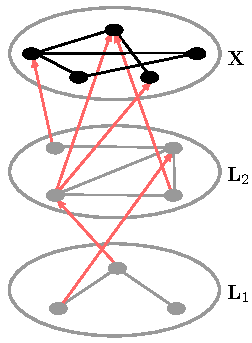
\includegraphics[height=.7\textheight]{latentmultilayer}}
\end{minipage}
\end{frame}

%%%%%%%%%%%%%%%%%%%%%%%%%%%%%%%%%%%%%%%%%%%%%%%%%%%%%%%%%%%%%%%%
\begin{frame}
\frametitle{Connections}

\begin{itemize}
\item Non-linear generalization of a factor model.

\vspace{1em}
\item A general version: $\BL_2 = f_1(\BL_1) + \BE$ etc. for unknown function $f_1$, has been proposed as Deep Latent Gaussian Model \citep{RezendeEtal14}.

\vspace{1em}
\item The choice $\phi(\BL^T \bfB) \equiv \phi(\BL)^T \bfB$ corresponds to Non-linear Gaussian belief networks \citep{FreyHinton99}.

\end{itemize}
\end{frame}
%%%%%%%%%%%%%%%%%%%%%%%%%%%%%%%%%%%%%%%%%%%%%%%%%%%%%%%%%%%%%%%%

\begin{frame}
\frametitle{Our plan}

Incorporate {\colbit sparse} estimation of the model parameters to model non-linear interactions.

\begin{center}
\includegraphics[width=.7\textwidth]{latentinteractions}
\end{center}

\visible<2>{
\begin{itemize}
\item Monte-Carlo EM to maximize a variational lower bound of the likelihood,

\item Theoretical properties of estimates
\end{itemize}
}
\end{frame}
%%%%%%%%%%%%%%%%%%%%%%%%%%%%%%%%%%%%%%%%%%%%%%%%%%%%%%%%%%%%%%%%

\begin{frame}
\frametitle{Conclusion}
\begin{itemize}
\onslide<2->{
\item We proposed a general framework to model data in {\colbit complex hierarchical structures}, with a focus on multi-level biological Omics datasets;
}
\onslide<3->{
\vspace{1em}
\item We provide an {\colbit estimation algorithm} and {\colbit testing methodology} for the parameters involved, with theoretical results ensuring the validity of the methods;
}
\onslide<4->{
\vspace{1em}
\item The general nature of the work leaves many {\colbit directions for future developments}.
}
\end{itemize}

\end{frame}
%%%%%%%%%%%%%%%%%%%%%%%%%%%%%%%%%%%%%%%%%%%%%%%%%%%%%%%%%%%%%%%%

\begin{frame}
\frametitle{References}
Preprint available at: \url{https://arxiv.org/abs/1803.03348}

\vspace{1em}
\onslide<2>
{\scriptsize
\bibliographystyle{apalike}
\bibliography{IISAbib}
}
\end{frame}
%%%%%%%%%%%%%%%%%%%%%%%%%%%%%%%%%%%%%%%%%%%%%%%%%%%%%%%%%%%%%%%%


\begin{frame}
\centering
{\huge\textcolor{UniBlue}{\textbf{THANK YOU!}}}\\

%\vspace{2em}
%
%{\colubf Questions?}
\end{frame}

\end{document}
